\documentclass{beamer}

\usepackage{graphicx} 
\usepackage{braket} 
\usepackage{tikz} 
\usepackage{quantikz} 
\usepackage{subcaption}
\usepackage{listings}
\usepackage{hyperref}

\bibliographystyle{plain}
\usetheme{Singapore} % Choose your preferred theme
\usecolortheme{lily}

% Title slide
\title{Exploring the Variational Quantum Eigensolver through an application on the Lipkin Model}
\author{Keran Chen}
\institute{University of Oslo}
\date{\today}

\AtBeginSection[]{
  \begin{frame}
    \vfill
    \centering
    \begin{beamercolorbox}[sep=8pt,center]{title}
      \usebeamerfont{title}\insertsectionhead\par%
    \end{beamercolorbox}
    \vfill
  \end{frame}
}


\newcommand{\sw}{\mathbf{SWAP}} 
\newcommand{\cnot}{\mathbf {CNOT}} 
\begin{document}

\begin{frame}
  \titlepage
\end{frame}


\section{Motivations}
\begin{frame}{Motivations}
  \begin{block}{Many-Body Problems}
  \begin{itemize}
	\item Want to find eigenvalues of Hamiltonian.
	\item Hilbert space of complex quantum systems grow exponentially with the number of particles.   
  \end{itemize}
  \end{block}

\begin{block}{Current Solutions}
\begin{itemize}
    \item Exact diagonalization: Limited to small system sizes due to computational complexity.
    \item Classical algorithms suffer from the exponential increase in Hilbert space as the system size increase.
  \end{itemize}
\end{block}
\end{frame}

\begin{frame}[t]
\begin{block}{Variational Quantum Eigensolver (VQE)}
\begin{itemize}
	\item Uses variational methods for finding the ground state energy of a system: $ E_0 \leq \braket{\psi|\hat H|\psi}$
	\item Allows the representation of quantum systems using limited number of qubits.
	\item Realisable in our noisy intermediate scale quantum computing (NISQ) era due its low depth circuit.
\end{itemize}	
\end{block}

\begin{block}{The Lipkin Model}
	\begin{itemize}
		\item Simple but non-trivial, has analytical solutions.
		\item A testbed for quantum simulation algorithms such as VQE
	\end{itemize}	
\end{block}
	
\end{frame}

\section{Quantum Computing}
\begin{frame}{Basis}

We choose the single qubit computational basis to be the eigenbasis of the Pauli Z matrix,
\[ \ket{0} = \begin{pmatrix} 1 \\ 0 \end{pmatrix} \quad \ket{1} = \begin{pmatrix} 0 \\ 1 \end{pmatrix}  \] 	
Multiqubit basis are tensor products of single qubits basis,
\[ 
\begin{aligned}
	\ket{00} = \ket{0} \otimes \ket{0} \\
	\ket{01} = \ket{0} \otimes \ket{1} \\
	\ket{10} = \ket{1} \otimes \ket{0} \\
	\ket{11} = \ket{1} \otimes \ket{1}
\end{aligned}
\] 
\end{frame}


\begin{frame}[t]
	\frametitle{Gates}	

\begin{block}{One Qubit Gates}
	\begin{itemize}
		\item X-gate$ X = \begin{pmatrix} 0 & 1 \\ 1 & 0 \end{pmatrix}  $ 
		\item Y-gate $ Y = \begin{pmatrix} 0 & -i \\ i & 0 \end{pmatrix}  $ 
		\item Z-gate $ Z = \begin{pmatrix} 1 & 0 \\ 0 & -1 \end{pmatrix}  $ 
		\item Hadamard gate: $ H = \frac{1}{\sqrt{2}} \begin{pmatrix} 1 & 1 \\ 1 & -1 \\ \end{pmatrix} $ 
		\item Phase gate $ S^{\dagger} = \begin{pmatrix} 1 & 0 \\ 0 & -i \end{pmatrix} $ 
		\item Rotation gates: $R_x(\theta)=\cos{\frac{\theta}{2}}I-\imath \sin{\frac{\theta}{2}}X, R_y(\phi)=\cos{\frac{\phi}{2}}I-\imath \sin{\frac{\phi}{2}}X.$
	\end{itemize}
\end{block}
\end{frame}

\begin{frame}[t]
\begin{block}{Two Qubit Gates}
	\begin{itemize}
		\item $ CNOT = \begin{pmatrix} 1 & 0 & 0 & 0 \\ 0 & 1 & 0 & 0 \\ 0 & 0 & 0 & 1 \\ 0 & 0 & 1 & 0 \end{pmatrix} $ 
		\item $ SWAP = \begin{pmatrix} 1 & 0 & 0 & 0 \\ 0 & 0 & 1 & 0 \\ 0 & 1 & 0 & 0 \\ 0 & 0 & 0 & 1 \end{pmatrix} $
	\end{itemize}
		
\end{block}

\begin{block}{Von Neumann entropy}
	It's a measure of entanglement
	\[ S(A,B)=-\mathrm{Tr}\left(\rho_{A,B}\log_2 (\rho_{A,B})\right). \] 
\end{block}
	
\end{frame}

\begin{frame}[t]
	\frametitle{Measurements}
	\begin{itemize}
		\item Computational basis is in the $ Z $ basis $ \implies $ must apply the appropriate uniform transformation to rotate the basis
		\item Measurement is a non-reversible operation $ \implies $ a new copy of the system must be prepared before each measurement.
		\item Measurement collapses the state onto one of the eigenstates $ \implies $ measure $ N $ times then divide by $N$  to reconstruct the coefficients following.
	\end{itemize}
	\begin{block}{Change of Basis}
		Since we write Hamiltonian in terms of the Pauli matrices, and the computational basis are in the $ Z, ZI, ZIII $  basis, measuring in other basis requires us to rotate the our computational basis to the appropriate basis, given by the unitary transformation below.
		\begin{align*}
			X &= HZH \\
			Y &= HS^{\dagger}ZHS
		\end{align*}
	\end{block}
\end{frame}

\section{Models}

\begin{frame}[t]
	\frametitle{One-Qubit System}
The Hamiltonian is given by:
	\[ H = H_0 + \lambda H_I \] 
where $ H_0 $ and $ H_I $ can be written in terms of the Pauli matrices as:
\begin{align*}
	H_I &= cI +\omega_z Z + \omega_x X, \\
	H_0 &= \mathcal{E} I + \Omega Z \\
\end{align*}
with $c = (V_{11}+V_{22})/2$, $\omega_z = (V_{11}-V_{22})/2$, $\omega_x = V_{12}=V_{21}$ and $\Omega = \frac{E_1-E_2}{2},$
We choose $E_1=0$, 
$E_2=4$, $V_{11}=-V_{22}=3$ and $V_{12}=V_{21}=0.2$.

\end{frame}


\begin{frame}[t]
	\frametitle{Two Qubit System}
Hamiltonian is again: 
\[H = H_0 + \lambda H_I \]
where $ H_0 $ and $ H_I $ can be written in terms of the Pauli matrices as
\[H_0 = a I\otimes I + b I\otimes Z + cZ\otimes I + dZ\otimes Z\]
with $a = 4, b = -0.75, c = -2.75, d = -0.5$
\[H_I =H_x \ X \otimes X +H_z \ Z \otimes Z, \]
with $Hx = 2.0,
Hz = 3.0$
\end{frame}


\begin{frame}[t]
	\frametitle{The Lipkin Model}
	\framesubtitle{J=1}
	\begin{itemize}
		\item N fermions distributed in two levels each having an N-fold degeneracy and separated by an energy $ \epsilon $. 
		\item Each state describe by $ \ket{n, \sigma} $ 
		\item Can be written in terms of quasispin operators $ J_{\pm} $ and $ J_z $.
	\end{itemize}
	\textbf{ The Lipkin Hamiltonian is }
	\[ H = H_0 + H_1(V) + H_2(W) \] 
	We will assume now $ W = 0 $ and $ H_2 = 0 $ 
\end{frame}
\begin{frame}
	In matrix representation, the Hamiltonian is:

	\[ H = 
	\begin{pmatrix}
		-\epsilon & 0 & v \\
		0 & 0 & 0 \\
		v & 0 & \epsilon
	\end{pmatrix} 
	\]

	Or in terms of Pauli matries:
	\[H =  \frac{\epsilon}{2} (ZI + IZ) + \frac{1}{2} V (XX - YY)\]

\end{frame}

\begin{frame}[t]
	\frametitle{The Lipkin Model}
	\framesubtitle{J=2}
	In matrix representation, the Hamiltonian is:
	\[H =
	\begin{pmatrix}
	-2\varepsilon & 0 & \sqrt{6}V & 0 & 0 \\
	0 & -\varepsilon + 3W & 0 & 3V & 0 \\
	\sqrt{6}V & 0 & 4W & 0 & \sqrt{6}V \\
	0 & 3V & 0 & \varepsilon + 3W & 0 \\
	0 & 0 & \sqrt{6}V & 0 & 2\varepsilon
\end{pmatrix} \]
For $ W = 0 $  in terms of Pauli matries:
\[\begin{aligned}
		H &= \epsilon\left( ZIII + IZII + IIZI + IIIZ \right) \\
		  &+ \frac{v}{2} (XXII + XIXI + XIIX + IXXI + IXIX + IIXX) \\
		  &- \frac{v}{2} (YYII + YIYI + YIIY + IYYI + IYIY + IIYY)
\end{aligned} \] 

\end{frame}

\begin{frame}[t]
	\frametitle{Level Mapping}
	\textbf{How to map the Fermions to qubits?} 
	\begin{block}{Direct Mapping}
		Map each state $ \ket{n, \sigma} $  by a qubit, with $ \ket{0} $ and $ \ket{1} $ representing the unoccupied state and occupied state respectively. 
		\begin{itemize}
			\item Requires $ 2N $ qubits for a system of $ N $ particle.
		\end{itemize}
	\end{block}
	\begin{block}{Level Mapping}
		Instead map 
		\[ 
		\begin{aligned}
			\ket{0} &\longleftrightarrow \ket{n, -1} \\
			\ket{1} &\longleftrightarrow \ket{n, +1}.
		\end{aligned}\] 
		\begin{itemize}
			\item Requires only $ N $ qubits for a system of $ N $ particle.
		\end{itemize}
	\end{block}
\end{frame}

\begin{frame}[t]
	\frametitle{The W Term}
	We rewrote $ H_2 $ in terms of the Pauli matrices and obtained:
	\[ 	
	\begin{aligned}
			H_2 &= \frac{1}{2}W ( 4IIII + 2 (XXII + XIXI + XIIX + IXXI + IXIX + IIXX \\ 
		&+ YYII + YIYI + YIIY + IYYI + IYIY + IIYY))
		\end{aligned}\]
where we represented the $ \hat N $ (particle number operator) by $ 4IIII $ since there are $ 4 $ particles in this system.
\end{frame}
\section{VQE}

\begin{frame}[t]
	\frametitle{VQE}
	The hybrid variational algorithm follows the following steps:
	\begin{enumerate}
	\item Prepare a parameterised quantum circuit (the ansatz) $|\Psi(\vec{\theta})\rangle$.
	\item Measure the expectation value $E(\vec{\theta})$.
	\item Use a classical optimization algorithm (gradient based or not) to update the parameters $\vec{\theta}$.
	\item Repeat the above steps until the change in $E(\vec{\theta})$ is below a certain threshold.	
	\end{enumerate}
\end{frame}

\begin{frame}[t]
	\frametitle{Implementation}
\begin{block}{Quantum Computing (\texttt{base.py})}
	\begin{itemize}
		\item Three classes: \texttt{Qubit, Qubits\_2(Qubit), Qubits(Qubits\_2)} 
		\item All single and two qubit gates mentioned above for any combination of qubits in the circuit.
		\item Measurement is done by calling \texttt{Qubits.measure(n\_shots)} which returns the counts of all states.
	\end{itemize}
\end{block}
	
\begin{block}{VQE}
	\begin{itemize}
		\item Class: \texttt{VQE(ansatz,expectation)}
		\item Minimisation algorithm: \texttt{scipy.optimize.minimise(method=``Powell'')}
	\end{itemize}

\end{block}
\end{frame}

\begin{frame}[t]
	\frametitle{Ansatz}
	\begin{block}{One-Qubit}
		\begin{figure}[ht]
	\centering
	\begin{quantikz}
    	\lstick{$q_0$}  &\gate{Rx(\theta)}   &\gate{Ry(\phi)} &\qw\\
	\end{quantikz}
	\caption{One-qubit ansatz}
	\label{fig:1an}
	
	\end{figure}
	\end{block}

	\begin{block}{Two-Qubit}
		\begin{figure}[ht]
	\centering
	\begin{quantikz}
		\lstick{$q_0$}  &\gate{Rx(\theta_0)}   &\gate{Ry(\phi_0)} &\targ{} &\qw\\
		\lstick{$q_1$}  &\gate{Rx(\theta_1)}   &\gate{Ry(\phi_1)} &\ctrl{-1} &\qw\\
	\end{quantikz}

	\caption{Two-qubit ansatz}
	\label{fig:2an}
	\end{figure}
	\end{block}
\end{frame}

\begin{frame}

\begin{block}{Four-Qubit}
	
	\begin{figure}[ht]
	\centering
	\begin{quantikz}
		\lstick{$q_0$}  &\gate{Rx(\theta_0)}   &\gate{Ry(\phi_0)} &\targ{} &\qw &\qw &\qw &\qw\\
		\lstick{$q_1$}  &\gate{Rx(\theta_1)}   &\gate{Ry(\phi_1)} &\ctrl{-1} &\qw &\targ{} &\qw &\qw \\
		\lstick{$q_2$}  &\gate{Rx(\theta_2)}   &\gate{Ry(\phi_2)} &\qw &\qw &\ctrl{-1} &\targ{} &\qw\\
		\lstick{$q_3$}  &\gate{Rx(\theta_3)}   &\gate{Ry(\phi_3)} &\qw &\qw &\qw  &\ctrl{-1} &\qw \\
	\end{quantikz}
	\caption{Four-qubit ansatz}
	\label{fig:4an}
\end{figure}	
	\end{block}
	
\end{frame}


\section{Results}
\begin{frame}[t]
	\frametitle{One-Qubit}

	\begin{figure}[ht]
		\centering
		\begin{subfigure}[b]{0.45\textwidth}
		\begin{center}
			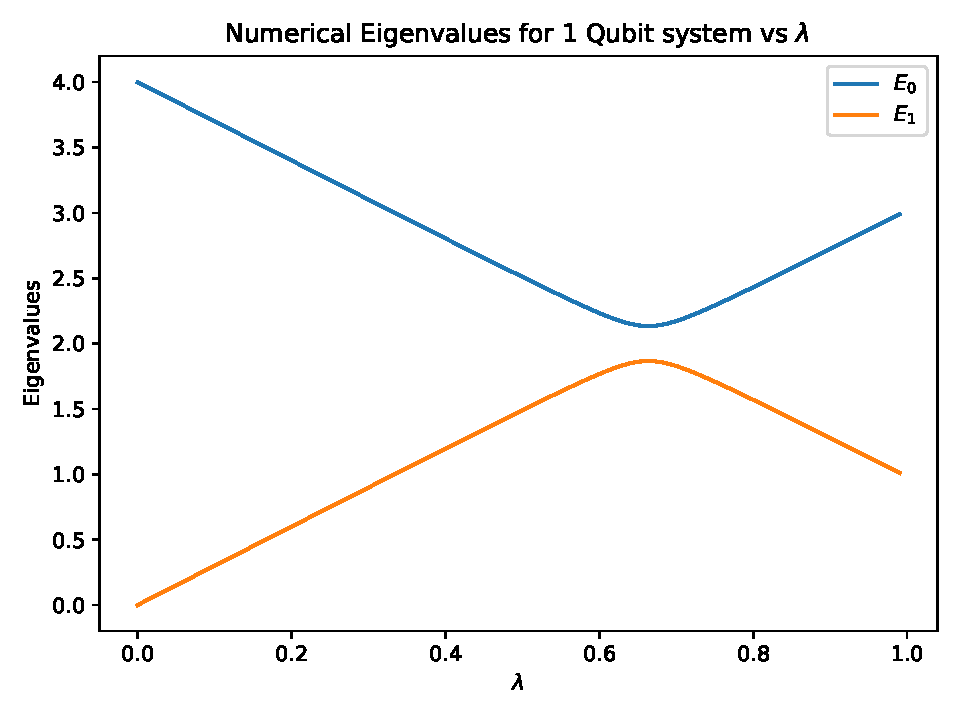
\includegraphics[width=\textwidth]{../src/plots/eigs-1-cl.pdf}
		\end{center}
		\caption{Classical eigenvalues as a function of the interaction strength $ \lambda $ , with colours denoting different energy levels.}
		\label{fig:eig-1}
		\end{subfigure}
		\hfill
		\begin{subfigure}[b]{0.45\textwidth}
		\begin{center}
			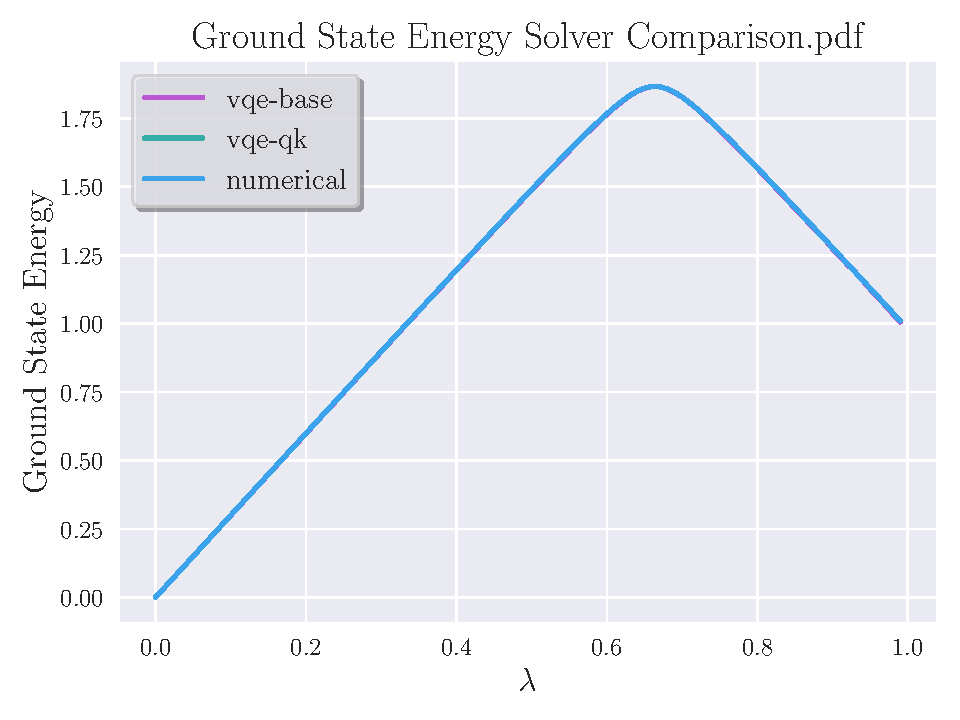
\includegraphics[width=\textwidth]{../src/plots/1qb-al.pdf}	
		\end{center}
		\caption{Ground state energy calculated using VQE for a one-qubit system as a function of $ \lambda $ , from both our implementation and Qiskit.}
		\label{fig:1-qb-all}
		\end{subfigure}
		\label{fig:1-qb}
	\end{figure}
	
\end{frame}

\begin{frame}[t]
	\frametitle{Two-Qubit}
	\begin{figure}[ht]
		\centering
		\begin{subfigure}[b]{0.45\textwidth}
		\begin{center}
			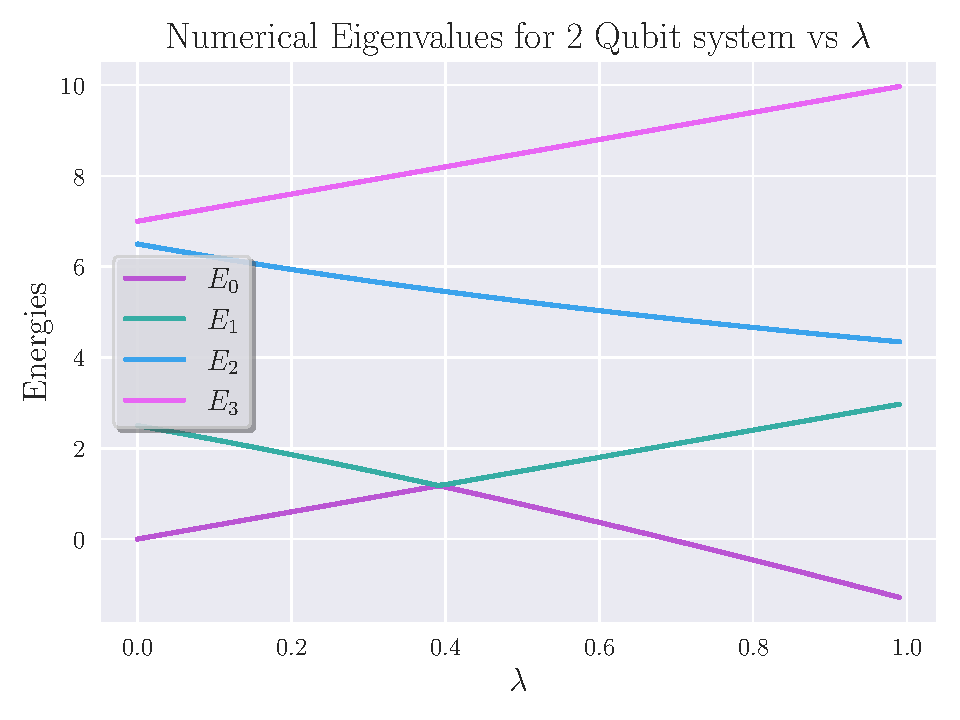
\includegraphics[width=\textwidth]{../src/plots/eigs-2-cl.pdf}
		\end{center}
		\caption{Numerical eigenvalues for a two-qubit system, with colours indicating distinct energy levels.}
		\label{fig:eig-2}
		\end{subfigure}
		\hfill
		\begin{subfigure}[b]{0.45\textwidth}
		\begin{center}
			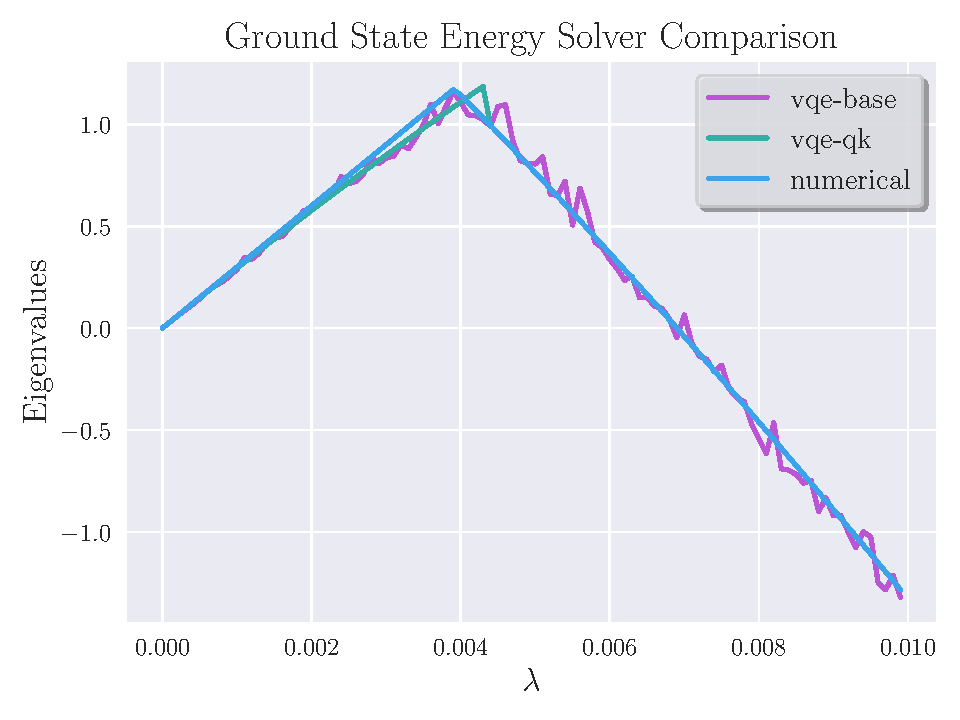
\includegraphics[width=\textwidth]{../src/plots/2qb-all.pdf}	
		\end{center}
		\caption{Ground state energy determined with VQE for a two-qubit system as a function of interaction strength $\lambda$, from both our implementation and Qiskit.}
		\label{fig:2-qb-all}
		\end{subfigure}
		\label{fig:2-qb}
	\end{figure}
\end{frame}

\begin{frame}[t]
	\frametitle{Two-Qubit}
	\framesubtitle{Von Neumann Entropy}
	\begin{figure}[ht]
		\centering
		\begin{subfigure}[b]{0.45\textwidth}
		\begin{center}
			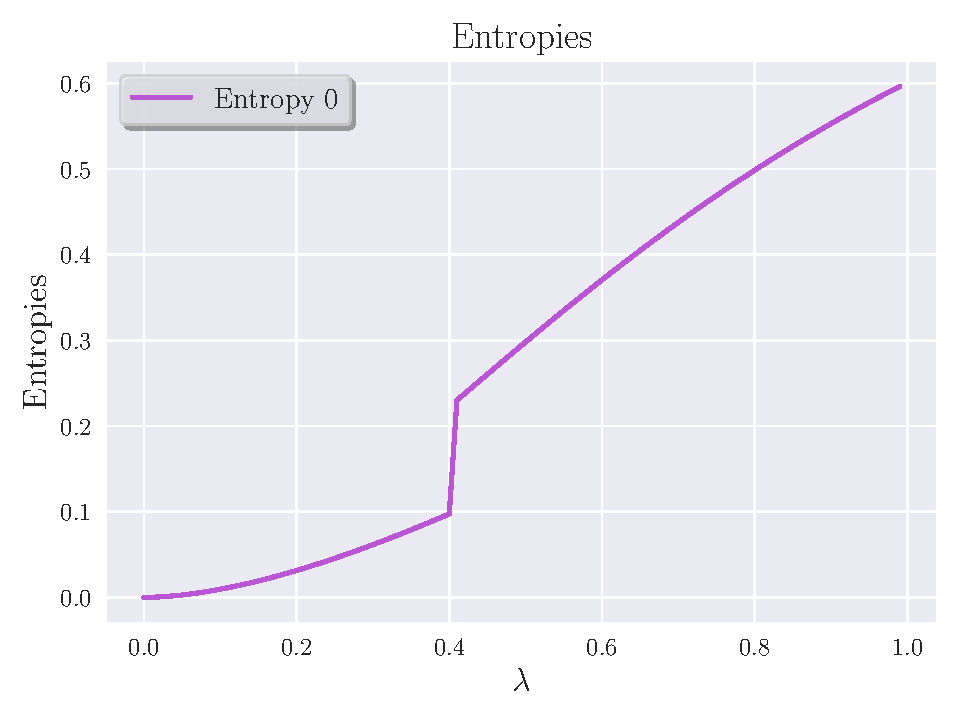
\includegraphics[width=\textwidth]{../src/plots/entropies-2-0.pdf}
		\end{center}
		\caption{Von Neumann entropy of the ground state for a simple two-qubit system as a function of interaction strength.}
		\label{fig:entropie-0}
		\end{subfigure}
		\hfill	
		\begin{subfigure}[b]{0.45\textwidth}
		\begin{center}
			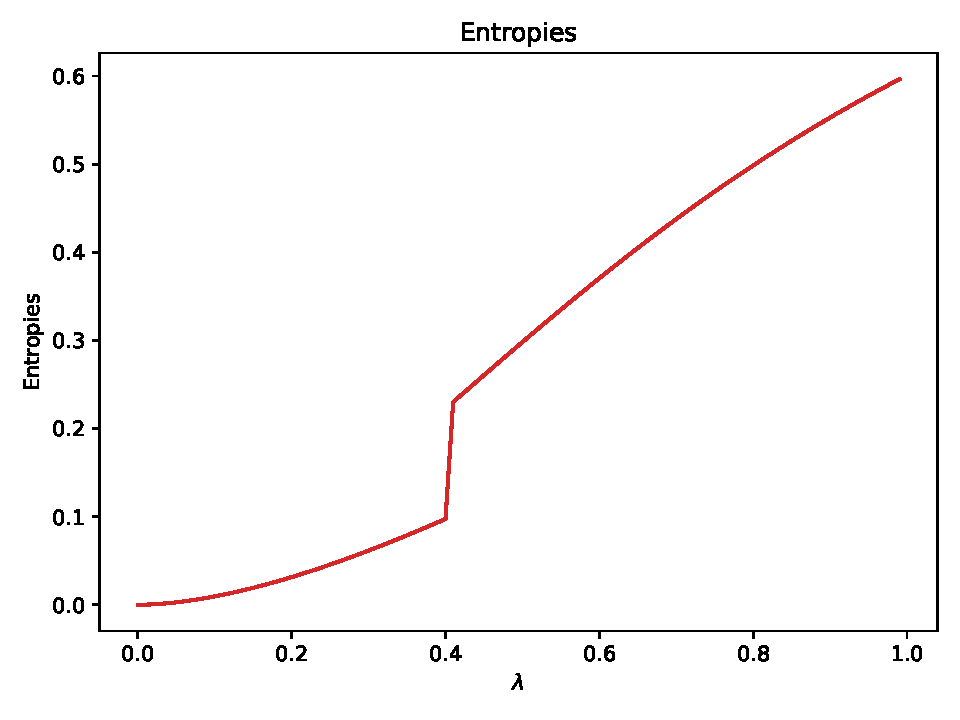
\includegraphics[width=\textwidth]{../src/plots/entropies-2-cl.pdf}
		\end{center}
		\caption{Von Neumann entropy of the ground state for a simple two-qubit
system as a function of interaction strength.}
		\label{fig:entropie-4}
		\end{subfigure}
			
		\label{fig:-src-plots-entropies-2-cl-pdf}
	\end{figure}
	
\end{frame}
\begin{frame}[t]
	\frametitle{Lipkin}
	\framesubtitle{J=1}
	\begin{figure}[ht]
		\centering
		\begin{subfigure}[b]{0.45\textwidth}
		\begin{center}
			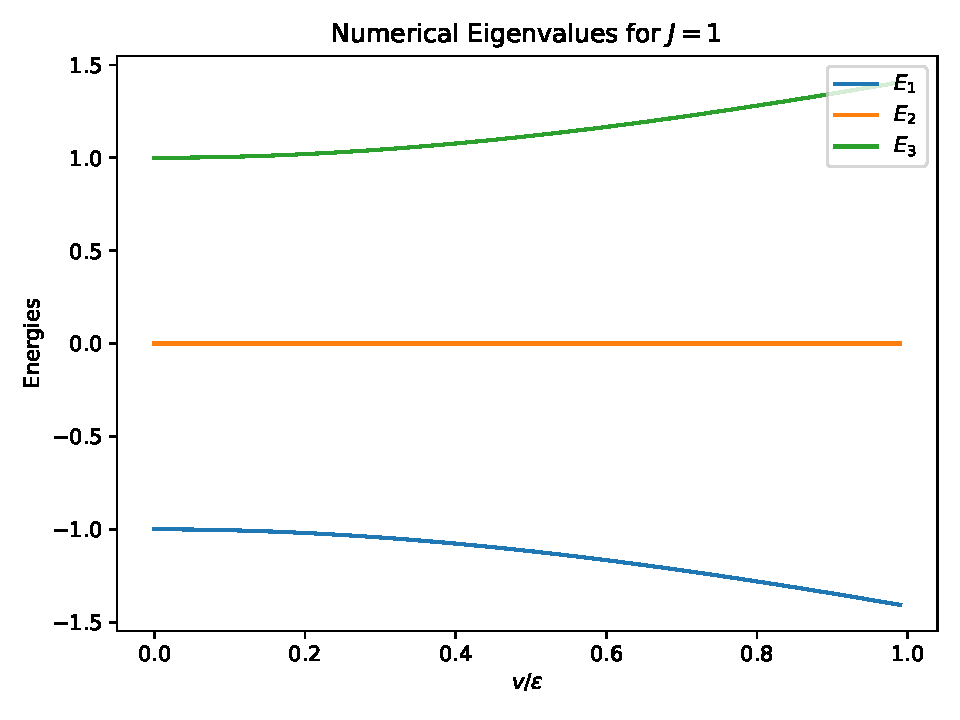
\includegraphics[width=\textwidth]{../src/plots/eigs-lipkin-2.pdf}
		\end{center}
		\caption{Numerical eigenvalues for a two-qubit system, with colours indicating distinct energy levels.}
		\label{fig:eig-lipkin-2}
		\end{subfigure}
		\hfill
		\begin{subfigure}[b]{0.45\textwidth}
		\begin{center}
			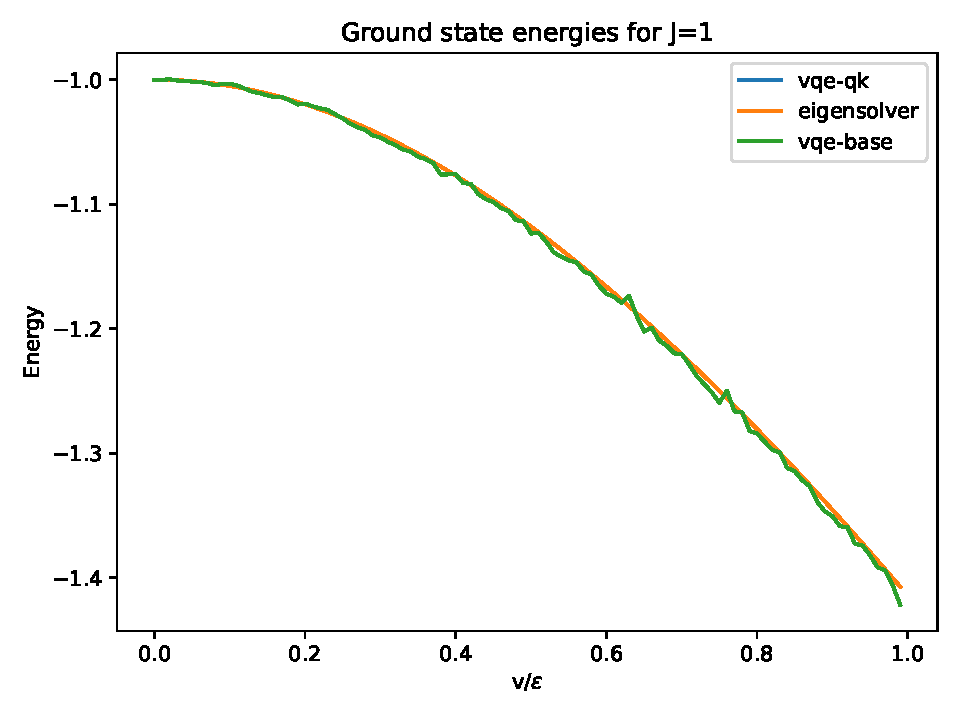
\includegraphics[width=\textwidth]{../src/plots/lipkin-2.pdf}	
		\end{center}
		\caption{Ground state energy determined with VQE for a two-qubit system as a function of interaction strength $\lambda$, from both our implementation and Qiskit.}
		\label{fig:2-qb-all}
		\end{subfigure}
		\label{fig:2-qb}
	\end{figure}
\end{frame}

\begin{frame}[t]
	\frametitle{Lipkin}
	\framesubtitle{J=2}
	\begin{figure}[ht]
		\centering
		\begin{subfigure}[b]{0.45\textwidth}
		\begin{center}
			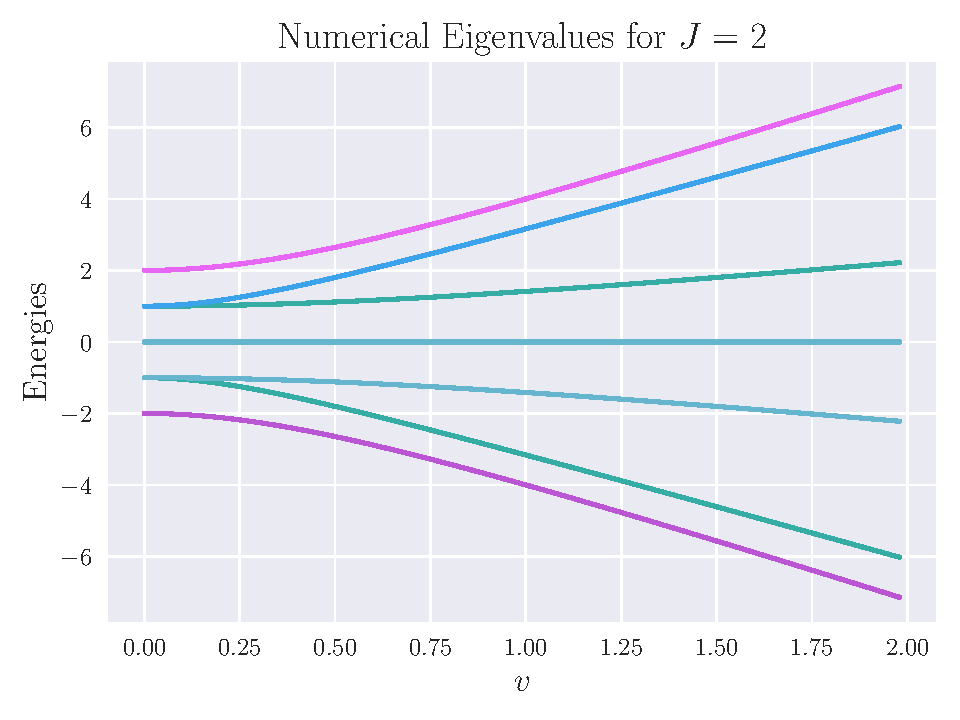
\includegraphics[width=\textwidth]{../src/plots/lipkin-eigs-4.pdf}
		\end{center}
		\caption{Numerical results for the Lipkin Model with $J = 2$, utilising the full Hamiltonian with size $16 \times 16$, where all energies have a degeneracy of $2$.}
		\label{fig:eig-lipkin-2}
		\end{subfigure}
		\hfill
		\begin{subfigure}[b]{0.45\textwidth}
		\begin{center}
			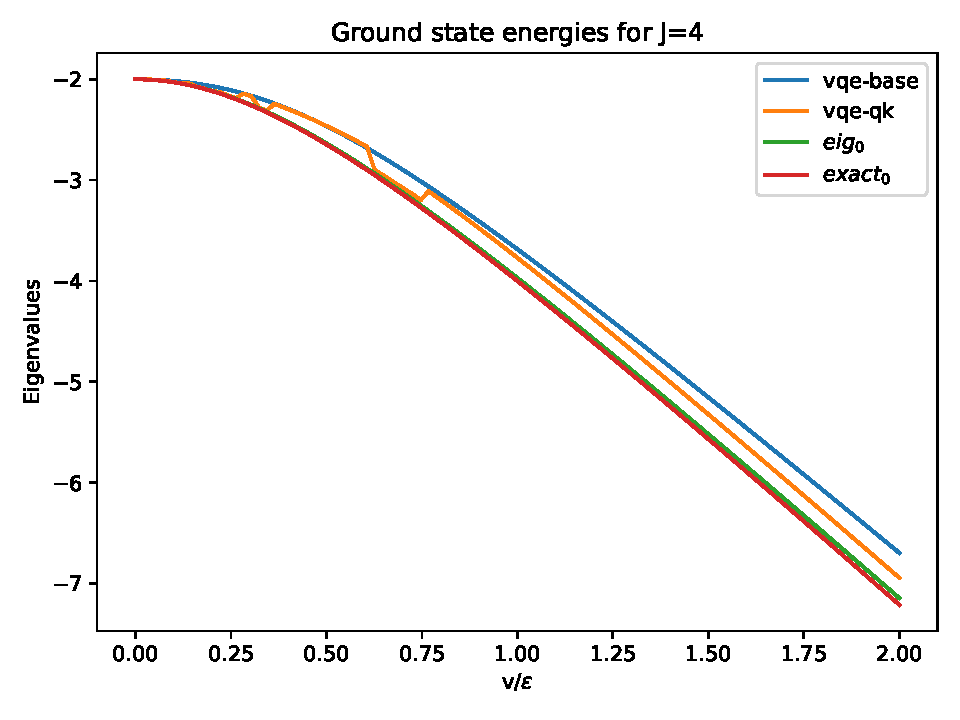
\includegraphics[width=\textwidth]{../src/plots/lipkin-4.pdf}	
		\end{center}
		\caption{Ground state energy determined with VQE for a two-qubit system as a function of interaction strength $\lambda$, from both our implementation and Qiskit.}
		\label{fig:2-qb-all}
		\end{subfigure}
		\label{fig:2-qb}
	\end{figure}
\end{frame}

\begin{frame}[t]
	\frametitle{Lipkin}
	\framesubtitle{J=2, with W}
	\begin{figure}[ht]
		\centering
		\begin{subfigure}[b]{0.45\textwidth}
		\begin{center}
			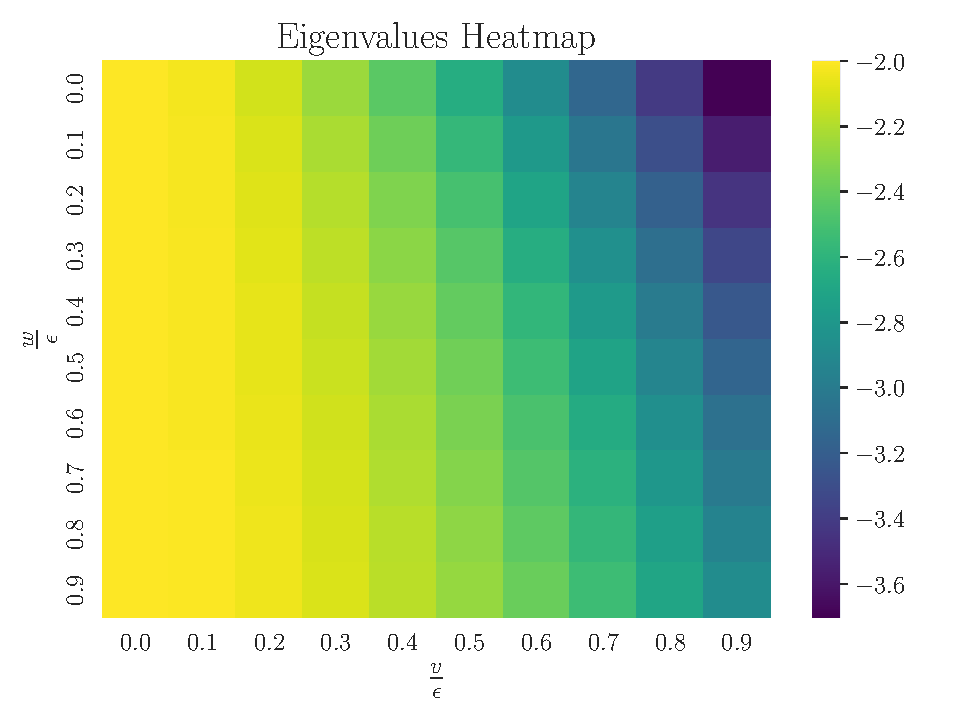
\includegraphics[width=\textwidth]{../src/plots/lipkin-w-eig.pdf}
		\end{center}
		\caption{Numerical results for the Lipkin Model for $ J=2 $ with the W term.}
		\end{subfigure}
		\hfill
		\begin{subfigure}[b]{0.45\textwidth}
		\begin{center}
			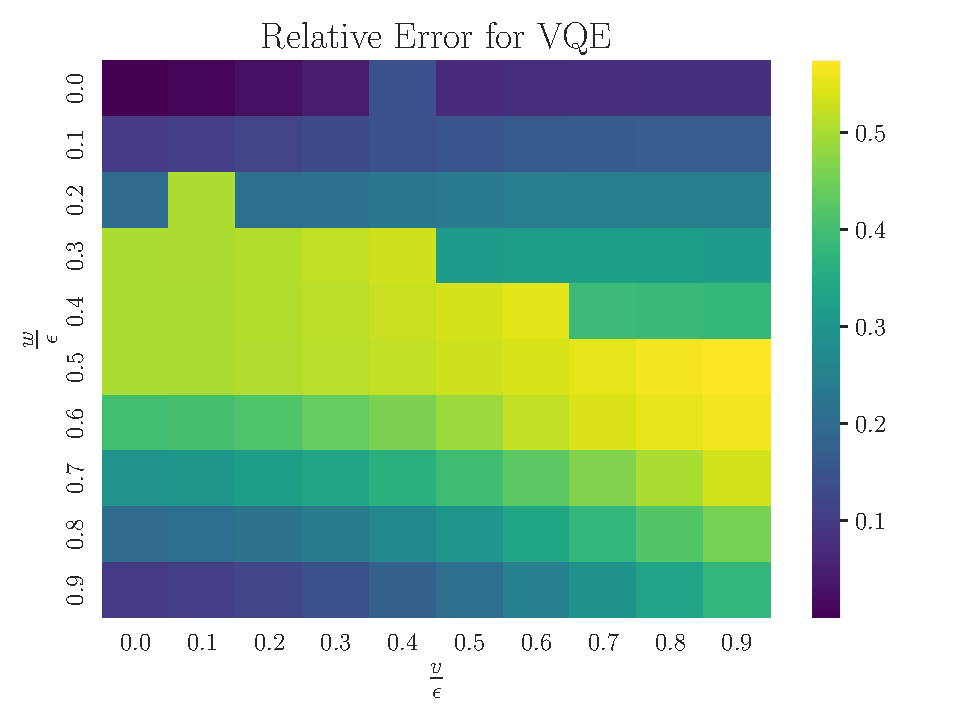
\includegraphics[width=\textwidth]{../src/plots/rel-error.pdf}	
		\end{center}
		\caption{Relative Error for Lipkin model for $ J=2 $ with W using qiskit.}
		\label{fig:2-qb-all}
		\end{subfigure}
		\label{fig:2-qb}
	\end{figure}
\end{frame}

	

\section{Discussion}
\begin{frame}[t]
	\frametitle{Increasing number of shots}
	\begin{figure}[ht]
		\centering
		\begin{subfigure}[b]{0.45\textwidth}
		\begin{center}
			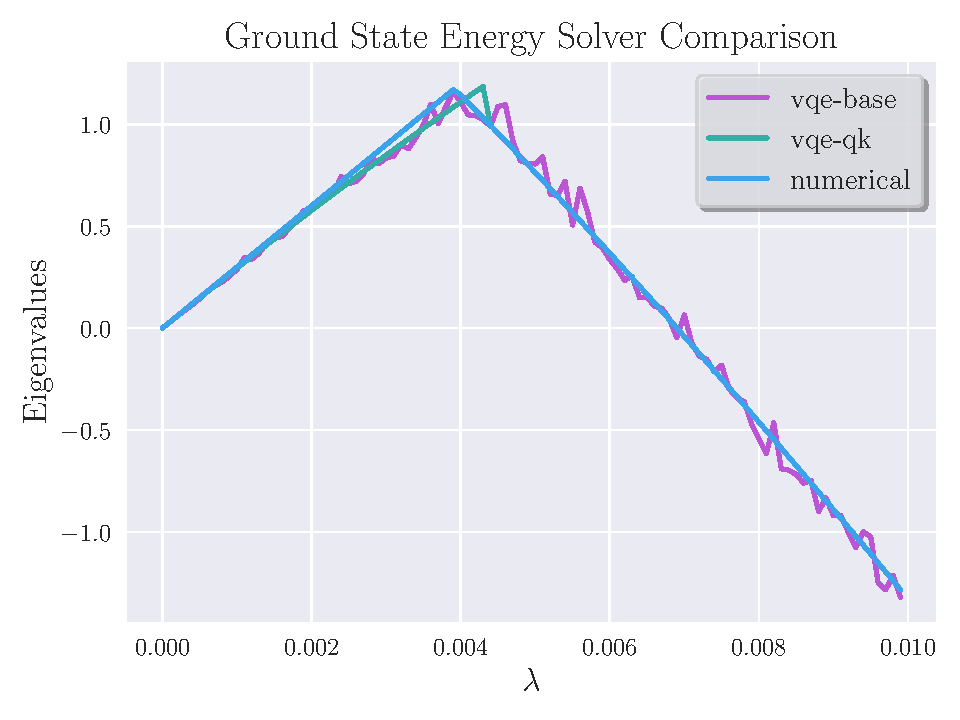
\includegraphics[width=\textwidth]{../src/plots/2qb-all.pdf}
		\end{center}
		\caption{round state energy determined with VQE for a two-qubit system as a function of interaction strength $\lambda$, from both our implementation and Qiskit.}
		\label{fig:2qb-all}
		\end{subfigure}
		\hfill
		\begin{subfigure}[b]{0.45\textwidth}
		\begin{center}
			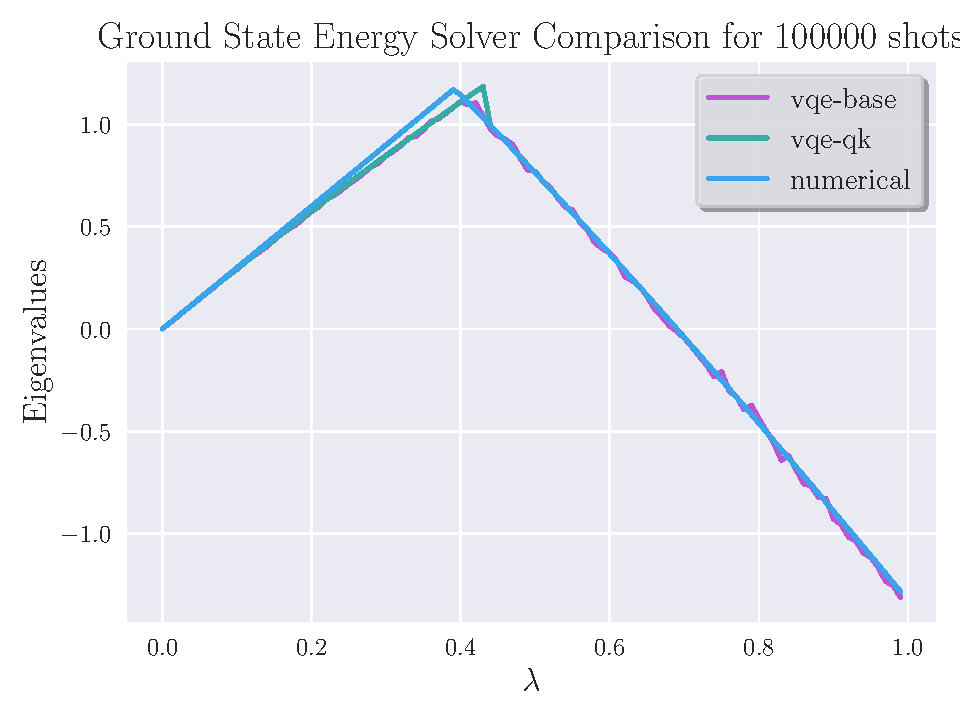
\includegraphics[width=\textwidth]{../src/plots/2qb-100000.pdf}	
		\end{center}
		\caption{Ground state energy determined with VQE for a two-qubit system as a function of interaction strength $\lambda$, with $ 100000 $ shots gate.}
		\label{fig:2-qb-all}
		\end{subfigure}
		\label{fig:2-qb}
	\end{figure}

	
\end{frame}
\begin{frame}[t]
	\frametitle{The Importance of Entanglement}

	\begin{figure}[ht]
		\centering
		\begin{subfigure}[b]{0.45\textwidth}
		\begin{center}
			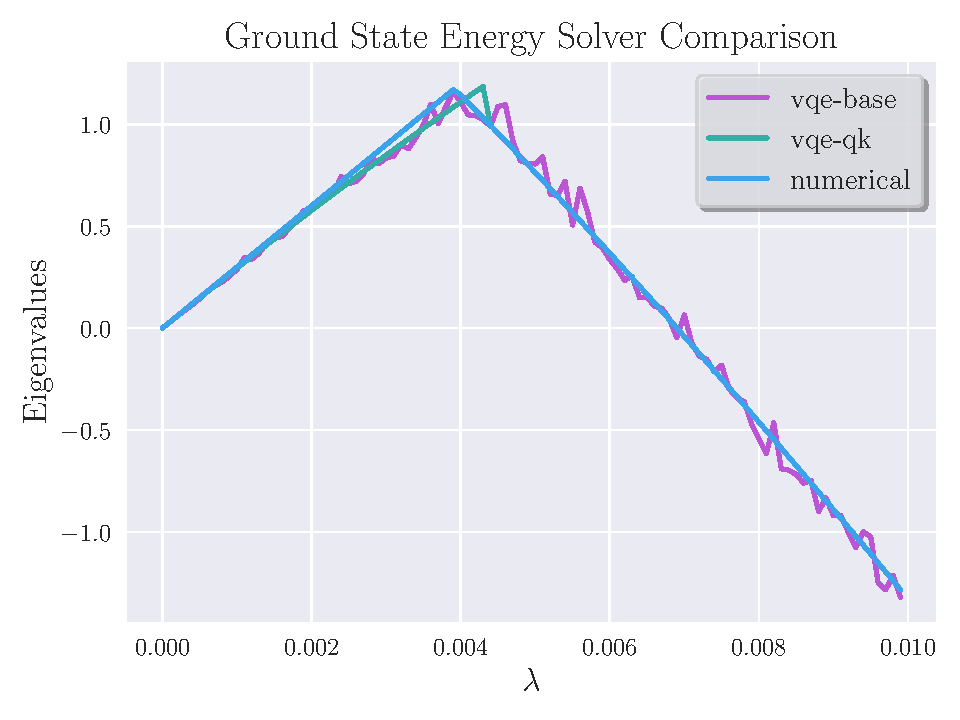
\includegraphics[width=\textwidth]{../src/plots/2qb-all.pdf}
		\end{center}
		\caption{round state energy determined with VQE for a two-qubit system as a function of interaction strength $\lambda$, from both our implementation and Qiskit.}
		\label{fig:2qb-all}
		\end{subfigure}
		\hfill
		\begin{subfigure}[b]{0.45\textwidth}
		\begin{center}
			\includegraphics[width=\textwidth]{../src/plots/2qb-fucked.pdf}	
		\end{center}
		\caption{Ground state energy determined with VQE for a two-qubit system as a function of interaction strength $\lambda$, without the CNOT gate.}
		\label{fig:2-qb-all}
		\end{subfigure}
		\label{fig:2-qb}
	\end{figure}

	
\end{frame}
\begin{frame}[t]
	\frametitle{Choice of Ansatz}
There is no universal way to choose an ansatz, and there is no unique ansatz.
	\begin{block}{Bad ansatzs}
		\begin{figure}[ht]
		\centering
		\begin{quantikz}
			\lstick{$q_0$}  &\gate{Rx(\theta_0)}   &\gate{Ry(\phi_0)} &\qw &\qw\\
			\lstick{$q_1$}  &\gate{Rx(\theta_0)}   &\gate{Ry(\phi_0)} & \qw &\qw\\
		\end{quantikz}

	\end{figure}

		\begin{figure}[ht]
		\centering
		\begin{quantikz}
			\lstick{$q_0$}  &\gate{Rx(\theta_0)}   &\gate{Ry(\phi_0)}  &\ctrl{1} &\qw\\
			\lstick{$q_1$}  &\qw &\qw &\targ{} &\qw\\		
		\end{quantikz}

	\end{figure}
	\end{block}

\end{frame}

\begin{frame}[t]
	\frametitle{Choice of Ansatz}

	\begin{figure}[ht]
		\centering
		\begin{subfigure}[b]{0.45\textwidth}
		\begin{center}
			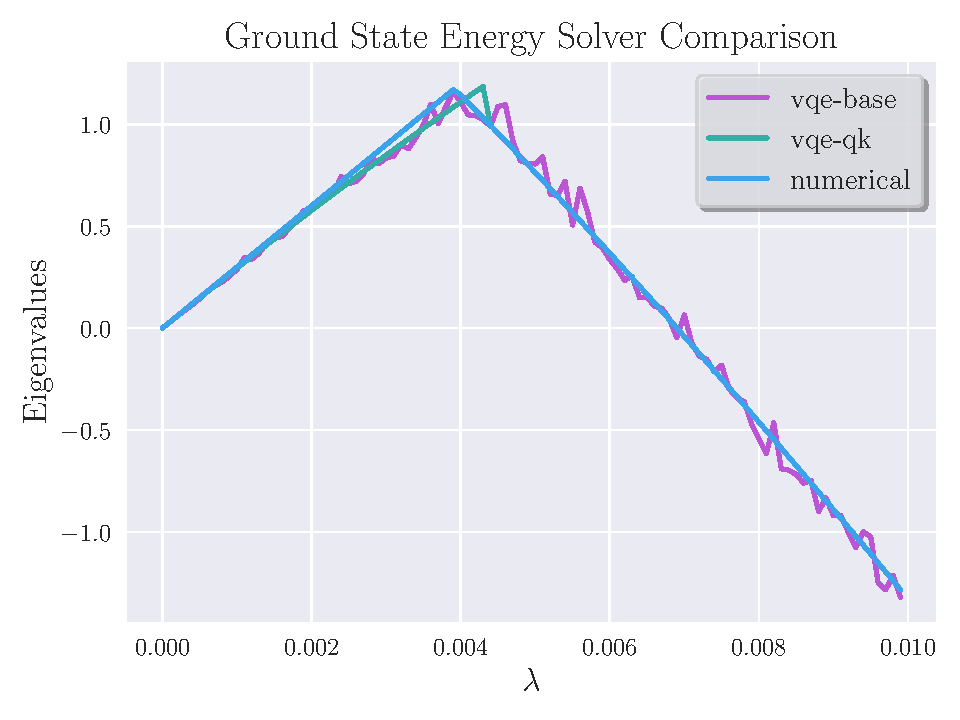
\includegraphics[width=\textwidth]{../src/plots/2qb-all.pdf}
		\end{center}
		\caption{round state energy determined with VQE for a two-qubit system as a function of interaction strength $\lambda$, from both our implementation and Qiskit.}
		\label{fig:2qb-all}
		\end{subfigure}
		\hfill
		\begin{subfigure}[b]{0.45\textwidth}
		\begin{center}
			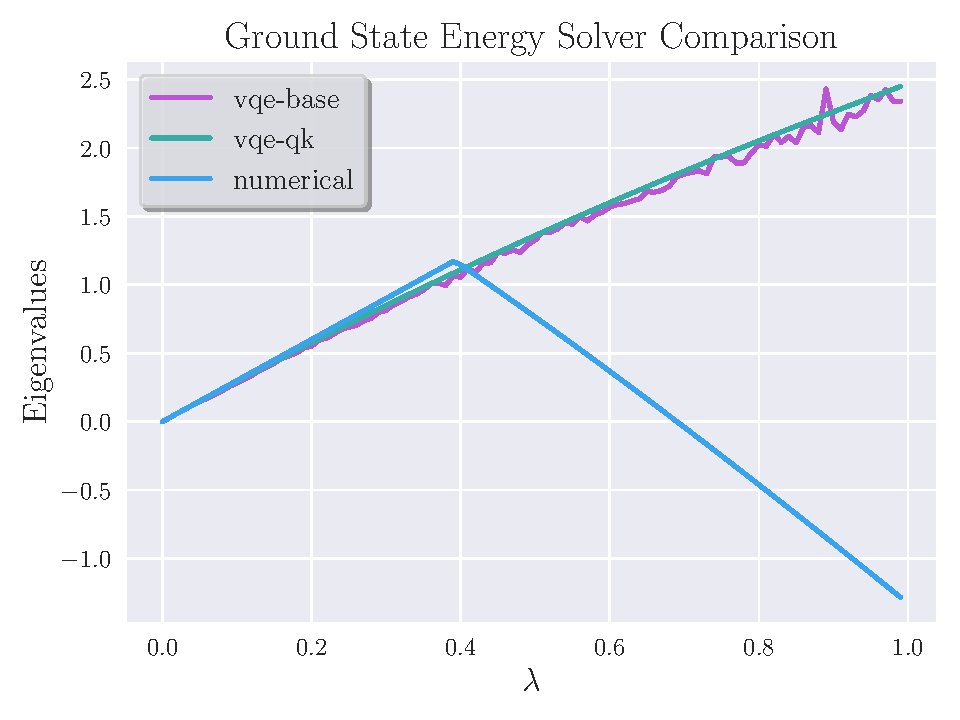
\includegraphics[width=\textwidth]{../src/plots/2qb-better.pdf}	
		\end{center}
		\caption{Ground state energy determined with VQE for a two-qubit system as a function of interaction strength $\lambda$, without the CNOT gate.}
		\label{fig:2-qb-all}
		\end{subfigure}
		\label{fig:2-qb}
	\end{figure}

	
\end{frame}
\begin{frame}[t]
	\frametitle{Ansatz Initialisation}
		\begin{itemize}
			\item Random
			\item Hartree Fock state \footnote{Jules Tilly, Hongxiang Chen, Shuxiang Cao, Dario Picozzi, Kanav Setia, Ying Li, Edward Grant, Leonard Wossnig, Ivan Rungger, George H. Booth, Jonathan Tennyson, "The Variational Quantum Eigensolver: a review of methods and best practices," arXiv:2111.05176 [quant-ph] (2021), accessed June 21, 2023, https://arxiv.org/abs/2111.05176.}
		\end{itemize}
\end{frame}
\begin{frame}[t]
	\frametitle{How Many Eigenvalues?}
	\begin{figure}[ht]
		\centering
		\begin{subfigure}[b]{0.45\textwidth}
		\begin{center}
			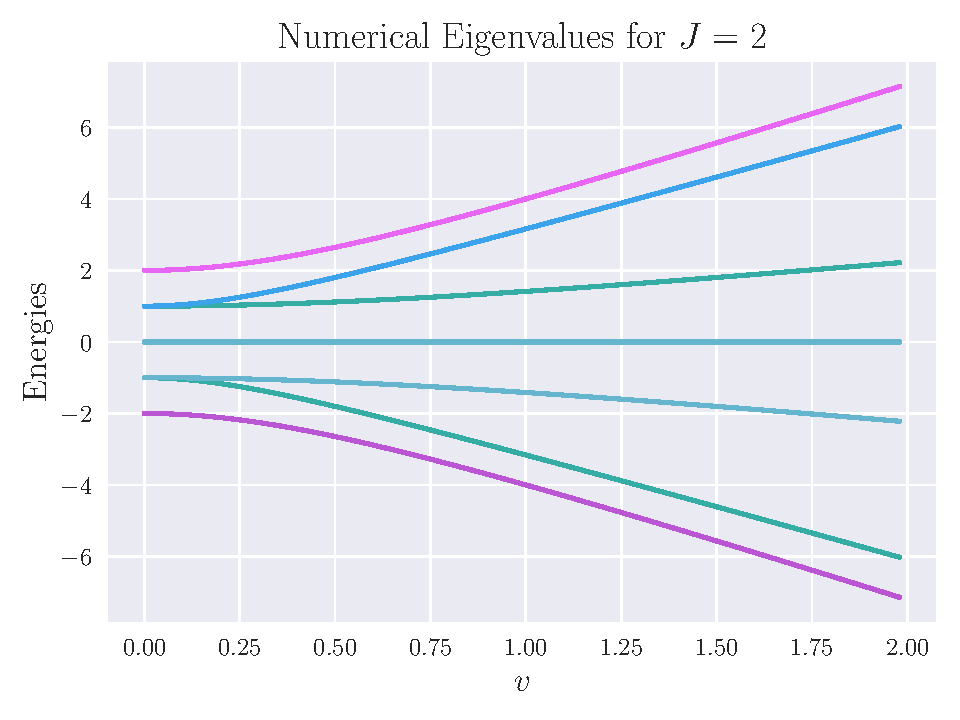
\includegraphics[width=\textwidth]{../src/plots/lipkin-eigs-4.pdf}
		\end{center}
		\caption{Energy eigenvalues for $ J=2 $ using the full Hamiltonian in terms of Pauli matrices}
		\label{fig:eig-lipkin-2}
		\end{subfigure}
		\hfill
		\begin{subfigure}[b]{0.45\textwidth}
		\begin{center}
			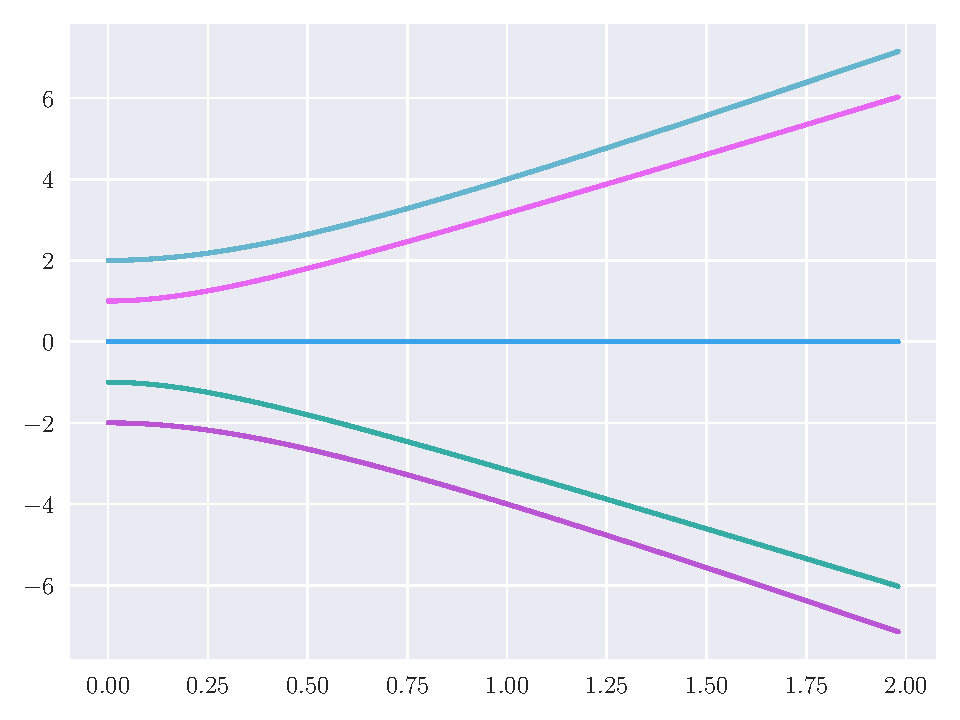
\includegraphics[width=\textwidth]{../src/plots/Eigen-5.pdf}	
		\end{center}
		\caption{Ground state energy for $ J=2 $  determined using the $ 5x5 $ matrix.}
		\label{fig:2-qb-all}
		\end{subfigure}
		\label{fig:2-qb}
	\end{figure}

	\begin{itemize}
		\item Different Encoding Scheme
		\item Non-allowed eigenenergies?
	\end{itemize}
\end{frame}

\begin{frame}[t]
	\frametitle{Performance}
	\begin{itemize}
		\item Same ansatz $ \implies $ converges to the same values (correct or not).
		\item Qiskit is faster and produces smoother graphs. 
		\item Non-gradient based methods (SLSQP, COBYLA, Powell) are faster than gradient based methods.
	\end{itemize}
	
\end{frame}

\section{Conclusion}
\begin{frame}{Conclusion}
  \begin{itemize}
	\item Simulation showed that the VQE is a promising algorithm for studying the ground state energy problem for the Lipkin Model.
	\item Including entanglement is essential for obtaining the correct results especially for when the ground state is highly entangled. 
	\item Non-gradient based methods are faster than gradient based methods
	\item Our implementation performs similar to the VQE from qiskit
\end{itemize}
\end{frame}

\begin{frame}[t]
	\frametitle{Future Work}
	\begin{itemize}
		\item Run on real quantum computers instead of a simulator.
		\item Compare the result from VQE with classical methods like HF or RPA.
		\item Implement general method for calculating expectation value through measurement.
		\item Test differential methods to initialise the ansatz
		\item Investigate the ground state energy for other systems.
		\item Investigate other choices of ansatz such as inclusion of multiple layers of gates.

	\end{itemize}
\end{frame}
\begin{frame}{Thank you!}
  \begin{center}
    \LARGE Questions?
  \end{center}
\end{frame}


\end{document}

